
\documentclass[pdf,
%8pt, 9pt, 10pt, 11pt, 12pt, 14pt, 17pt, 20pt
serif,
%handout,	% remove overlays
compress,
xcolor=table,
dvipsnames,
spanish,
aspectratio=169]{beamer}

\usepackage[algosection,lined]{algorithm2e}
\usepackage{minted}
\usepackage{tcolorbox}
\usepackage{xcolor}
\usepackage{comment}
\usepackage{todonotes}
\tcbuselibrary{minted}
\definecolor{bg}{rgb}{0.95,0.95,0.95}

%% Encoding, fonts, language
%%% Font & Encoding
\usepackage{libertine}
\usepackage[libertine]{newtxmath}
\usepackage[scaled=0.8]{beramono}  % for monospaced font
\usepackage{microtype}		% micro-typographic aspects of the fonts
\usepackage[T1]{fontenc}	% special fonts, e.g. for German umlaute
%% incompabtible with Biblatex
% \usepackage{ucs}
% \usepackage[utf8x]{inputenc}
%% compatible with Biblatex
\usepackage[utf8]{inputenc}



%% Language
%\usepackage[german]{babel}
%\usepackage{german}
\usepackage[english]{babel}


 
\usepackage{graphics}
\usepackage{url}
\usepackage{amsmath,amssymb,amsfonts,marvosym}
\usepackage{ulem}			% to cross out text
\usepackage{subfig}			% to cross out text
\normalem
\usepackage{ragged2e}
\let\raggedright=\RaggedRight
%%%%%%%%%%%%%%%%%%%%%%%%%
%   BEAMER SETTINGS    % 
%%%%%%%%%%%%%%%%%%%%%%%%

%\usefonttheme{serif}
%\renewcommand*{\ttdefault}{cmtt}

\definecolor{HHUblue}{HTML}{006AB3}
\setbeamercolor{structure}{fg=HHUblue}
\definecolor{backroundMinted}{HTML}{006293}
\definecolor{LightGray}{gray}{0.80}

\hypersetup{colorlinks,linkcolor=green,urlcolor=blue}

\setbeamerfont{frametitle}{family=\sffamily}
\setbeamerfont{title}{family=\sffamily}
\setbeamerfont{block title}{family=\sffamily}

%\usetheme{Copenhagen} % Boadilla
\usetheme{Warsaw}
\usecolortheme[rgb={0,0.4,0}]{structure}

\usecolortheme{default}   % beaver
\usefonttheme{default}		% default | professionalfonts | serif | structurebold | structureitalicserif | structuresmallcapsserif
\useinnertheme{default} 	% circles | default | inmargin | rectangles | rounded
\useoutertheme{default}	% default | infolines | miniframes | shadow | sidebar | smoothbars | smoothtree | split | tree

%\setbeamercovered{transparent}				% for transparent overlays
\setbeamercovered{invisible}				% for non-transparent overlays
\setbeamertemplate{navigation symbols}{}	% no navigation symbols
\setbeamertemplate{headline}[default]		% no headline
\setbeamertemplate{footline}[frame number]
\setbeamertemplate{section in toc}[]
\setbeamertemplate{subsection in toc}[]
\setbeamertemplate{itemize items}[square]
\setbeamertemplate{enumerate items}[square]
%\setbeamertemplate{blocks}[default]		% rectangular blocks
%\setbeamersize{text margin left=10pt,text margin right=10pt}

%% Bibliography style (http://tex.stackexchange.com/questions/97615/article-style-bibliography-in-beamer-class)
\setbeamertemplate{frametitle continuation}[from second]
% Now get rid of all the colours
\setbeamercolor*{bibliography entry title}{fg=black}
\setbeamercolor*{bibliography entry author}{fg=black}
\setbeamercolor*{bibliography entry location}{fg=black}
\setbeamercolor*{bibliography entry note}{fg=black}
% and kill the abominable icon
\setbeamertemplate{bibliography item}{\insertbiblabel}  % insert label from bib(la)tex
\AtBeginDocument{
  \renewcommand*{\bibfont}{\scriptsize}
}

%\tikzset{% makes available \only and \alt inside paths
%  only/.code args={<#1>#2}{\only<#1>{\pgfkeysalso{#2}}},
%  alt/.code args={<#1>#2#3}{\alt<#1>{\pgfkeysalso{#2}}{\pgfkeysalso{#3}}}
%}

\setbeamertemplate{footline}
{
  \leavevmode%
  \hbox{%
    \pgfsetfillopacity{0}\begin{beamercolorbox}[wd=.333333\paperwidth,ht=2.25ex,dp=1ex,left]{author in head/foot}%
      \usebeamerfont{author in head/foot}\pgfsetfillopacity{1}\color{gray}\hspace*{2ex}\insertshortauthor~~(\insertshortinstitute)
    \end{beamercolorbox}%
    \pgfsetfillopacity{0}\begin{beamercolorbox}[wd=.333333\paperwidth,ht=2.25ex,dp=1ex,center]{title in head/foot}%
      %\usebeamerfont{title in head/foot}\pgfsetfillopacity{1}\insertshorttitle
    \end{beamercolorbox}%
    \pgfsetfillopacity{0}\begin{beamercolorbox}[wd=.333333\paperwidth,ht=2.25ex,dp=1ex,right]{date in head/foot}%
      \usebeamerfont{date in head/foot}\pgfsetfillopacity{1}\insertshortdate{}\color{gray}\hspace*{2em}
      \insertframenumber{} %/ \inserttotalframenumber
      \hspace*{2ex}
    \end{beamercolorbox}}%
  \vskip0pt%
}


\newcommand{\separationframe}[1]{
\begin{frame}
\frametitle{}

\begin{center}
  \LARGE 
  \settowidth{\stmueTmp}{ #1 }
    \begin{minipage}{\stmueTmp}
    \begin{block}{}
    \begin{center}
    %\usebeamercolor[fg]{frametitle}
    #1
    \end{center}
    \end{block}
    \end{minipage}
\end{center}

\end{frame}
}

\newcommand\framecite[1]{
\vskip-2ex
\hfill #1%
\vskip-3.3ex ~
}

%\usepackage[
  hyperref=true,
  url=true,
  natbib=true,  
  %style=bst/biblatex-sp-unified,
  style=ieee,
  %citestyle=\mycitestyle,
  %refsection=chapter,
  maxbibnames=99,
  isbn=false,
  doi=false,
  eprint=false,
  backend=biber,
  %backend=bibtex,
  % sorting=ydnt,  % sort in descending chronological order
  indexing=cite,
  labelnumber,  % for numeric bibliography in beamer
  %toc=bib    % make bibliography appear in toc, incompatible with beamer
]{biblatex}   % bibliography

\addbibresource[datatype=bibtex]{references.bib}

\newcommand{\insertBib}{
  \printbibliography[
    %notkeyword=this
    ] 
}


\usepackage{datetime}
\newdateformat{specialdate}{\twodigit{\THEDAY}-\twodigit{\THEMONTH}-\THEYEAR}
%\newdateformat{specialdate}{\twodigit{\THEDAY}-\THEYEAR}
\date{\specialdate\today}

%%%%%%%%%%%%%%%%%%%%%%%%%%%%%%%%%%%%%%%%%%%%%%%%%%%%%%%%%%%%%%%%%
% HEADER
%%%%%%%%%%%%%%%%%%%%%%%%%%%%%%%%%%%%%%%%%%%%%%%%%%%%%%%%%%%%%%%%%

%\title[\arabic{page} ]{Advanced Computer Graphics}
\title[Arrays]{Jetpack Compose Tutorial}
% Sin subtitulos
\subtitle[short]{Mobile Programming}
% Corchetes: Solo apellidos de los integrantes, Llaves: Los nombres completos!!
\author[-]{Marco Aurelio Nuño-Maganda, Ph. D}
\institute[UPV]{Polytechnic University of Victoria}
\date[]{May-August 2024}
\logo{\pgfimage[width=1cm,height=1cm]{graphics/logo_upv_transparente}}			% Logo on all slides (pdf,png,jpg,eps)
%\titlegraphic{
\includegraphics[height=1.5cm]{graphics/logo_upv_transparente} \hfil \includegraphics[height=1.8cm]{graphics/c++.png}}	% Logo on title slide
\titlegraphic{
\includegraphics[height=1.5cm]{graphics/logo_upv_transparente} \hfill  
\includegraphics[height=1.5cm]{graphics/kotlin.png}}	% Logo on title slide



%%%%%%%%%%%%%%%%%%%%%%%%%%%%%%%%%%%%%%%%%%%%%%%%%%%%%%%%%%%%%%%%%
% SLIDES
%%%%%%%%%%%%%%%%%%%%%%%%%%%%%%%%%%%%%%%%%%%%%%%%%%%%%%%%%%%%%%%%%

% Configuracion para dibujar AUTOMATAS
\usepackage{tikz}
\usetikzlibrary{shadows,arrows.meta}
\usetikzlibrary{shadows,positioning,arrows}

\tikzset{parent/.style={align=center,text width=2cm,fill=green!20,rounded corners=2pt},
    child/.style={align=center,text width=2.8cm,fill=green!50,rounded corners=6pt},
    grandchild/.style={fill=pink!50,text width=2.3cm}
}
\usetikzlibrary{automata, positioning, arrows}


% ACtualizacion 2024: Se necesita esta Entrada
\newcommand{\rutaImagenes}{}

\begin{document}







\begin{frame}
    \titlepage
\end{frame}



<<<<<<< HEAD
%\renewcommand{\rutaImagenes}{Estudiante1/imgs}
%

\begin{frame}
\frametitle{Introduction to Android}
\begin{itemize}
\item Android is a Mobile OS
\item Nowadays, Android controls more than 80\% of the market Worldwide
\end{itemize}

\end{frame}



\begin{frame}
\frametitle{Android's History}
\begin{itemize}
\item Android is related to version of high carbohidrates cakes
\item Android was acquired by Google in 2005
\end{itemize}

\begin{center}

\includegraphics[width=4cm]{\rutaImagenes/funny-futurama-quotes-3.jpg}
\end{center}


\end{frame}



%\renewcommand{\rutaImagenes}{Estudiante2/imgs}
%

\begin{frame}
\frametitle{Introduction to Android}
\begin{itemize}
\item Android is a Mobile OS
\item Nowadays, Android controls more than 80\% of the market Worldwide
\end{itemize}

\end{frame}



\begin{frame}
\frametitle{Android's History}
\begin{itemize}
\item Android is related to version of high carbohidrates cakes
\item Android was acquired by Google in 2005
\end{itemize}

\begin{center}

\includegraphics[width=4cm]{\rutaImagenes/funny-futurama-quotes-3.jpg}
\end{center}


\end{frame}


=======
<<<<<<< HEAD
\renewcommand{\rutaImagenes}{Estudiante1/imgs}


\begin{frame}
\frametitle{Introduction to Android}
\begin{itemize}
\item Android is a Mobile OS
\item Nowadays, Android controls more than 80\% of the market Worldwide
\end{itemize}

\end{frame}



\begin{frame}
\frametitle{Android's History}
\begin{itemize}
\item Android is related to version of high carbohidrates cakes
\item Android was acquired by Google in 2005
\end{itemize}

\begin{center}

\includegraphics[width=4cm]{\rutaImagenes/funny-futurama-quotes-3.jpg}
\end{center}


\end{frame}



\renewcommand{\rutaImagenes}{Estudiante2/imgs}


\begin{frame}
\frametitle{Introduction to Android}
\begin{itemize}
\item Android is a Mobile OS
\item Nowadays, Android controls more than 80\% of the market Worldwide
\end{itemize}

\end{frame}



\begin{frame}
\frametitle{Android's History}
\begin{itemize}
\item Android is related to version of high carbohidrates cakes
\item Android was acquired by Google in 2005
\end{itemize}

\begin{center}

\includegraphics[width=4cm]{\rutaImagenes/funny-futurama-quotes-3.jpg}
\end{center}


\end{frame}


=======
%\renewcommand{\rutaImagenes}{Estudiante1/imgs}
%

\begin{frame}
\frametitle{Introduction to Android}
\begin{itemize}
\item Android is a Mobile OS
\item Nowadays, Android controls more than 80\% of the market Worldwide
\end{itemize}

\end{frame}



\begin{frame}
\frametitle{Android's History}
\begin{itemize}
\item Android is related to version of high carbohidrates cakes
\item Android was acquired by Google in 2005
\end{itemize}

\begin{center}

\includegraphics[width=4cm]{\rutaImagenes/funny-futurama-quotes-3.jpg}
\end{center}


\end{frame}



%\renewcommand{\rutaImagenes}{Estudiante2/imgs}
%

\begin{frame}
\frametitle{Introduction to Android}
\begin{itemize}
\item Android is a Mobile OS
\item Nowadays, Android controls more than 80\% of the market Worldwide
\end{itemize}

\end{frame}



\begin{frame}
\frametitle{Android's History}
\begin{itemize}
\item Android is related to version of high carbohidrates cakes
\item Android was acquired by Google in 2005
\end{itemize}

\begin{center}

\includegraphics[width=4cm]{\rutaImagenes/funny-futurama-quotes-3.jpg}
\end{center}


\end{frame}


>>>>>>> c3645c6 (Primer Commit)
>>>>>>> 9eaaac3 (Primer CommitXX)


\end{document}


\begin{frame}[fragile]
    \frametitle{Original XML Code}    


\begin{columns}
\column{0.65\linewidth}


    \begin{minted}[fontsize=\tiny]{xml}
<?xml version="1.0" encoding="utf-8"?>
<LinearLayout xmlns:android="http://schemas.android.com/apk/res/android"
    xmlns:app="http://schemas.android.com/apk/res-auto"
    xmlns:tools="http://schemas.android.com/tools"
    android:layout_width="match_parent"  android:layout_height="match_parent"
    android:orientation="vertical"  tools:context=".MainActivity">

    <TextView
        android:layout_width="match_parent" android:layout_height="0dp"
        android:layout_weight="2" android:text="Short text"
        android:gravity="center" android:background="#ffff00"  />

    <TextView
        android:layout_width="match_parent" android:layout_height="0dp"
        android:layout_weight="2"  android:gravity="center"
        android:id="@+id/TV1" android:background="#ff0000"
        android:text="Extremely long text giving the width of its siblings" />

    <TextView
        android:background="#ff00ff" android:layout_width="match_parent"
        android:layout_height="0dp" android:layout_weight="2"
        android:gravity="center" android:id="@+id/TV2"
        android:text="Medium length text"  />

</LinearLayout>

    \end{minted}
\column{0.35\linewidth}
\begin{itemize}
\item We have an activity with three \emph{TextViews} in a vertically oriented \textit{LinearLayout}, distributed at the top of the application, each one with the same weight to obtain the same size.
\end{itemize}
\end{columns}

    
\end{frame}

\begin{frame}
\frametitle{Composable Functions in Android}

Compasable Function:
\begin{itemize}
\item is a modern way of developing UI in Android. It is a Kotlin function that is annotated with @Composable
\item The @Composable annotation tells the Compose compiler that the functions is meant for UI construction. 
\item Unlike tradition XML layouts in Android, Composable functions allow us to build UI with Kotlin code which is more intuitive and flexible.
\item if we annotate this with @Composable, this now becomes a composable function.
\end{itemize}
Compose modifiers - allow you to decorate or augment a composable. 
\begin{itemize}
\item Change the composable's size, layout, behavior, and appearance
\item Add information, like accessibility labels
\item Process user input
\item Add high-level interactions, like making an element clickable, scrollable, draggable, or zoomable
\end{itemize}
\end{frame}




\begin{frame}[fragile]
    \frametitle{Main Activity of a Kotlin App using Composables}
\begin{minted}[fontsize=\tiny]{Kotlin}
class MainActivity : ComponentActivity() {
    override fun onCreate(savedInstanceState: Bundle?) {
        super.onCreate(savedInstanceState)
        setContent {
            // no need to load the UI, we just call the composable function
            FirstComposable()
        }
    }
}
\end{minted}
\end{frame}




\begin{frame}[fragile]
    \frametitle{First Compsable}
\begin{columns}
\column{0.55\linewidth}
\begin{minted}[fontsize=\tiny]{Kotlin}
@Composable
fun FirstComposable() {
    // state variables
    var enteredAmount by remember { mutableStateOf("") }
    var amountToSend by remember { mutableStateOf("0") }
    
    // Composable function that arranges 
	//child composables in a vertical sequence
    // This is similar to LinearLayout with 
	// vertical orientation in traditional Android XML Layout
    Column {
        // Composable function similar to TextView
        Text(text = amountToSend, fontSize = 18.sp)        
        // Composable function similar to EditText
        TextField(value = enteredAmount, onValueChange = {
            enteredAmount = it
        }, label = {
            Text(text = "Enter amount")
        })        
        // Composable function
        Button(onClick = { amountToSend = enteredAmount }) {
            Text(text = "Send Amount")
        }
    }
}
\end{minted}
\column{0.45\linewidth}
\begin{itemize}
\item Composable functions can use the remember API to store an object in memory. 
\item A value computed by remember is stored in the Composition during initial composition, and the stored value is returned during recomposition. 
\item \emph{remember} can be used to store both mutable and immutable objects.
\end{itemize}
\end{columns}
\end{frame}


\begin{frame}[fragile]
    \frametitle{Component Hierarchy}
 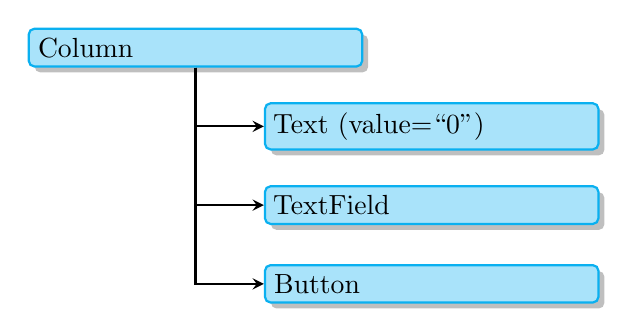
\begin{tikzpicture}[
text width=4cm,
ar/.style={->,>=stealth,thick},
every node/.style={rectangle,rounded corners=2pt,drop shadow,draw=ProcessBlue,fill=ProcessBlue!35,thick}]
    \node (n0) {Column};
    \node (n1) at (0,-1.0) [xshift=3cm] {Text (value=``0'')};
    \node (n2) at (0,-2) [xshift=3cm] {TextField};
    \node (n3) at (0,-3.0) [xshift=3cm] {Button};
    %\node (n4) at (0,-6) [xshift=6cm] {long text \\overflowing the shape};
    %\node (n5) at (0,-7.5) [xshift=6cm] {long text \\overflowing the shape};
    % Conecta Nodo 0=>1, 0=>2, 0=>3, 3=>4 y 3=>5
    %\foreach \ns/\ne in{0/1,0/2,0/3,3/4,3/5}
    \foreach \ns/\ne in{0/1,0/2,0/3}
    \draw[ar] (n\ns) |- (n\ne);
    \end{tikzpicture}

\end{frame}


\begin{frame}[fragile]
    \frametitle{Conversion to Jetpack Compose (1)}
    \begin{minted}[fontsize=\tiny]{Kotlin}
class MainActivity : ComponentActivity() {
    override fun onCreate(savedInstanceState: Bundle?) {
        super.onCreate(savedInstanceState)
        setContent {
            FirstComposeAppTheme {
                // A surface container using the 'background' color from the theme
                Surface(
                    modifier = Modifier.fillMaxSize(),
                    color = MaterialTheme.colorScheme.background
                ) {
                    LinearLayout1()
                    //LinearLayout2()
                    //LinearLayout3()
                }
            }
        }
    }
}
\end{minted}    
\end{frame}


\begin{frame}[fragile]
    \frametitle{Conversion to Jetpack Compose (2)}
\begin{columns}
\column{0.75\linewidth}

    \begin{minted}[fontsize=\tiny]{Kotlin}
fun LinearLayout1() {
    // Modification 1
    // 1 Column with Three rows ---
    Column(Modifier.width(IntrinsicSize.Max)) {
        Box(Modifier.fillMaxWidth().background(Color.Gray).weight(2.0f)) {
            Text("Short text")
        }
        Box(Modifier.fillMaxWidth().background(Color.Yellow).weight(2.0f)) {
            Text("Extremely long text giving the width of its siblings")
        }
        Box(Modifier.fillMaxWidth().background(Color.Green).weight(2.0f)) {
            Text("Medium length text")
        }
    }
}
\end{minted}

\column{0.20\linewidth}
\begin{center}
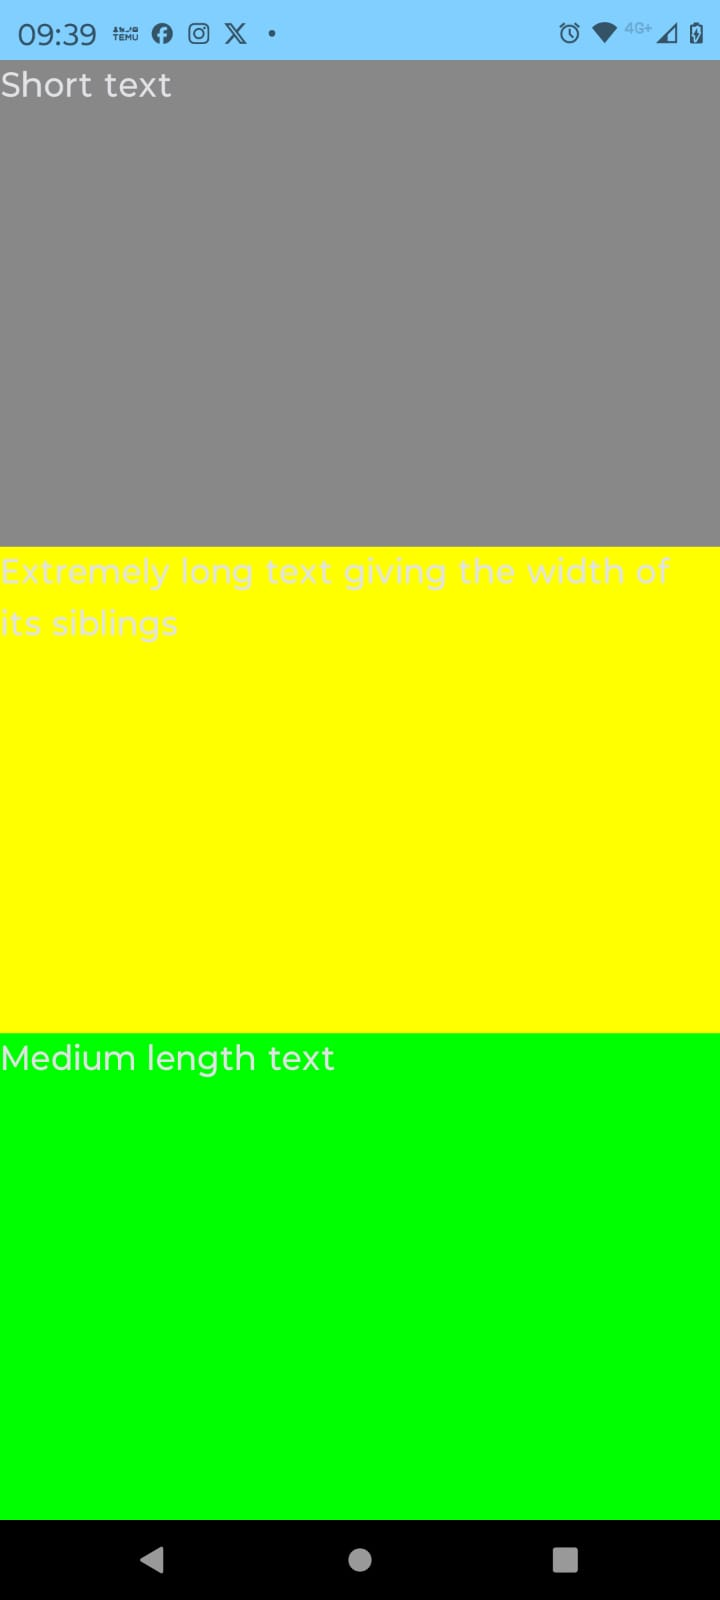
\includegraphics[width=0.98\columnwidth]{graphics/Screenshot1.jpg}    
\end{center}

\end{columns}



    
\end{frame}


\begin{frame}[fragile]
    \frametitle{Component Hierarchy}
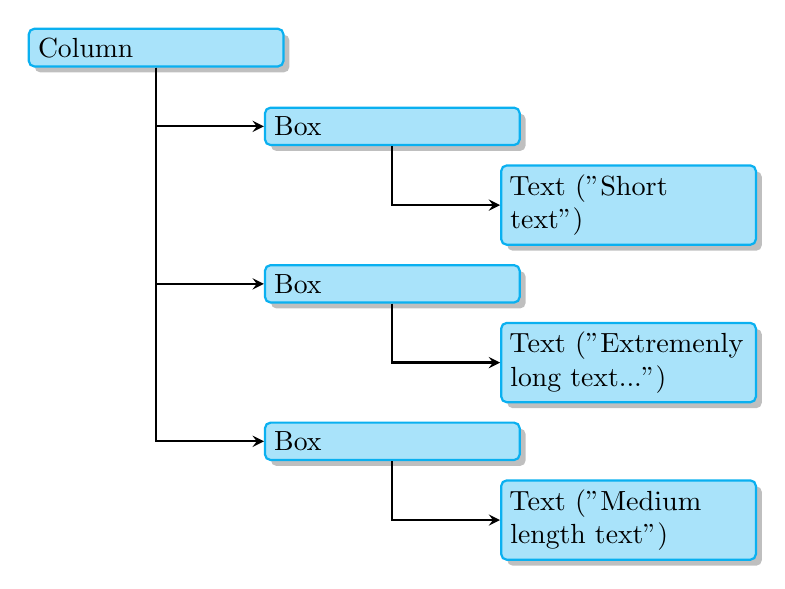
\begin{tikzpicture}[
text width=3cm,
ar/.style={->,>=stealth,thick},
every node/.style={rectangle,rounded corners=2pt,drop shadow,draw=ProcessBlue,fill=ProcessBlue!35,thick}]
    \node (n0) {Column};
    \node (n1) at (0,-1.0) [xshift=3cm] {Box};
    \node (n2) at (0,-2)   [xshift=6cm] {Text ("Short text")};
    \node (n3) at (0,-3.0) [xshift=3cm] {Box};
    \node (n4) at (0,-4.0) [xshift=6cm] {Text ("Extremenly long text...")};
    \node (n5) at (0,-5.0) [xshift=3cm] {Box};
    \node (n6) at (0,-6.0) [xshift=6cm] {Text ("Medium length text")};
    % Conecta Nodo 0=>1, 0=>2, 0=>3, 3=>4 y 3=>5
    %\foreach \ns/\ne in{0/1,0/2,0/3,3/4,3/5}
    \foreach \ns/\ne in{0/1,1/2,0/3,3/4,0/5,5/6}
    \draw[ar] (n\ns) |- (n\ne);
    \end{tikzpicture}



\end{frame}


\begin{frame}
    \frametitle{Explanation of the Conversion}

    \begin{itemize}
         \item The \texttt{ConstraintLayout} in XML is converted to a \texttt{Box} in Jetpack Compose.
        \item The \texttt{fillMaxSize()} function makes the \texttt{Box} occupy the entire available space, similar to \texttt{match\_parent}.
        \item The \texttt{contentAlignment = Alignment.Center} centers the text inside the \texttt{Box}, mimicking the \texttt{ConstraintLayout} constraints.
        \item The \texttt{TextView} is converted to \texttt{BasicText} with the text "Hello World!".    \end{itemize}

\end{frame}


\begin{frame}[fragile]
    \frametitle{Conversion to Jetpack Compose (3)}
\begin{columns}
\column{0.75\linewidth}

    \begin{minted}[fontsize=\tiny]{Kotlin}
fun LinearLayout2() { // Modification 2
	Row (Modifier.height(IntrinsicSize.Max)) {
		Box(Modifier.fillMaxHeight().background(Color.Gray).
			weight(2.0f).wrapContentSize(Alignment.Center)) {
			Text("Que es ñonga pregunto la Debayle?")
		}
		Box(Modifier.fillMaxHeight().background(Color.Red).
			weight(2.0f).wrapContentSize(Alignment.Center)) {
			Text("Le estaca no paraba de reir")
		}
    }
}
\end{minted}

\column{0.20\linewidth}
\begin{center}
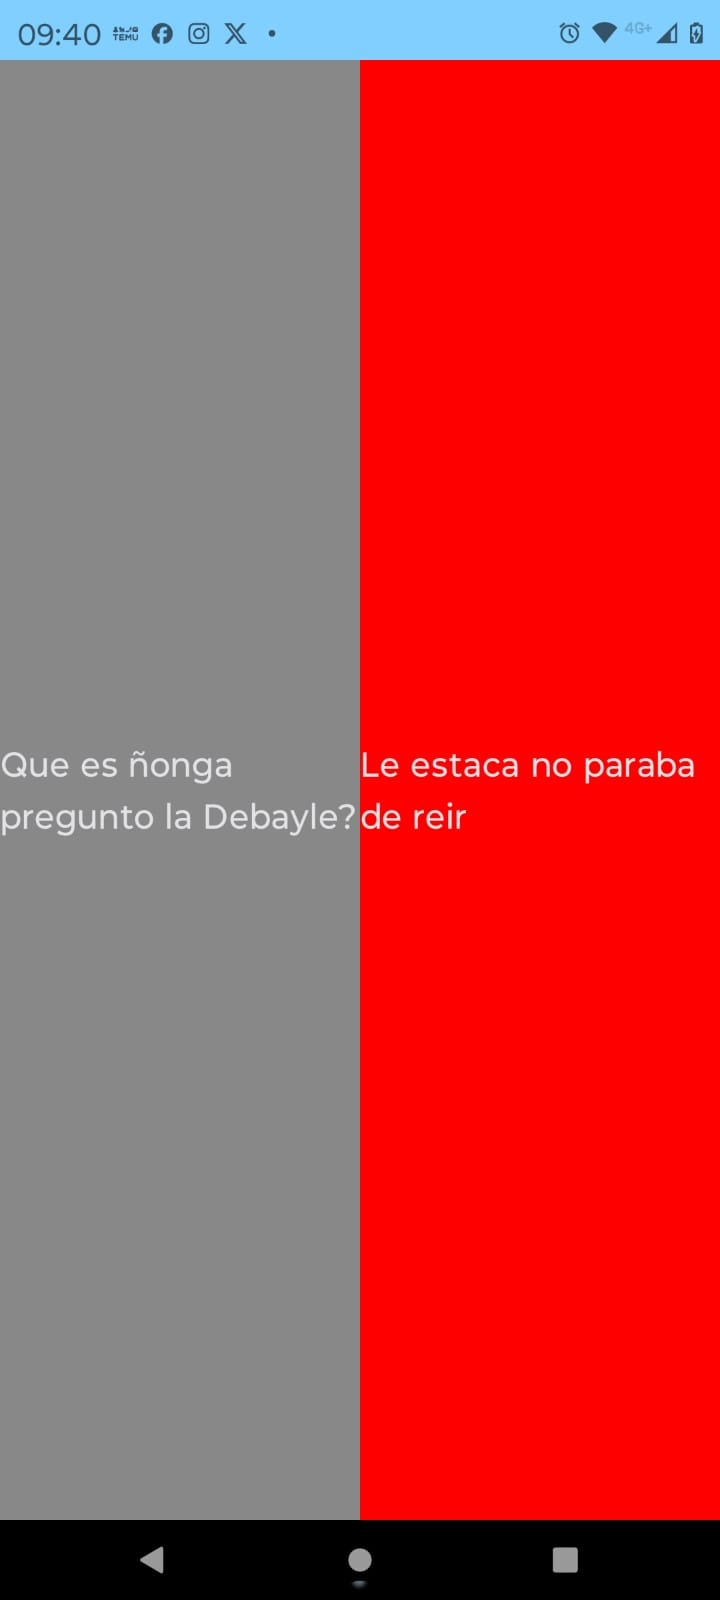
\includegraphics[width=0.98\columnwidth]{graphics/Screenshot2.jpg}    
\end{center}
\end{columns}



    
\end{frame}

\begin{frame}[fragile]
    \frametitle{Nested layouts}
\begin{columns}
\column{0.75\linewidth}

    \begin{minted}[fontsize=\tiny]{Kotlin}
fun LinearLayout3() {
    // Modification3 
    Row (Modifier.height(IntrinsicSize.Max)) {
        Box(Modifier.fillMaxHeight().background(Color.Gray)
                .weight(2.0f)
                .wrapContentSize(Alignment.Center)) {
            Column(Modifier.width(IntrinsicSize.Max)) {
                Box(Modifier.fillMaxWidth()
                    .background(Color.Gray)
                    .weight(2.0f).wrapContentSize(Alignment.Center)) {
                    Text("Short text")
                }
                Box(Modifier.fillMaxWidth()
                    .background(Color.Yellow)
                    .weight(2.0f).wrapContentSize(Alignment.Center)) {
                    Text("Extremely long text giving the width of its siblings")
                }
                Box(Modifier.fillMaxWidth()
                    .background(Color.Green)
                    .weight(2.0f).wrapContentSize(Alignment.Center)) {
                    Text("Medium length text")
                }
            }
        }
        Box(Modifier.fillMaxHeight().background(Color.Red)
            .weight(2.0f).wrapContentSize(Alignment.Center)) {
            Text("Le estaca no paraba de reir")
        }
    }
}
\end{minted}
\column{0.20\linewidth}
\begin{center}
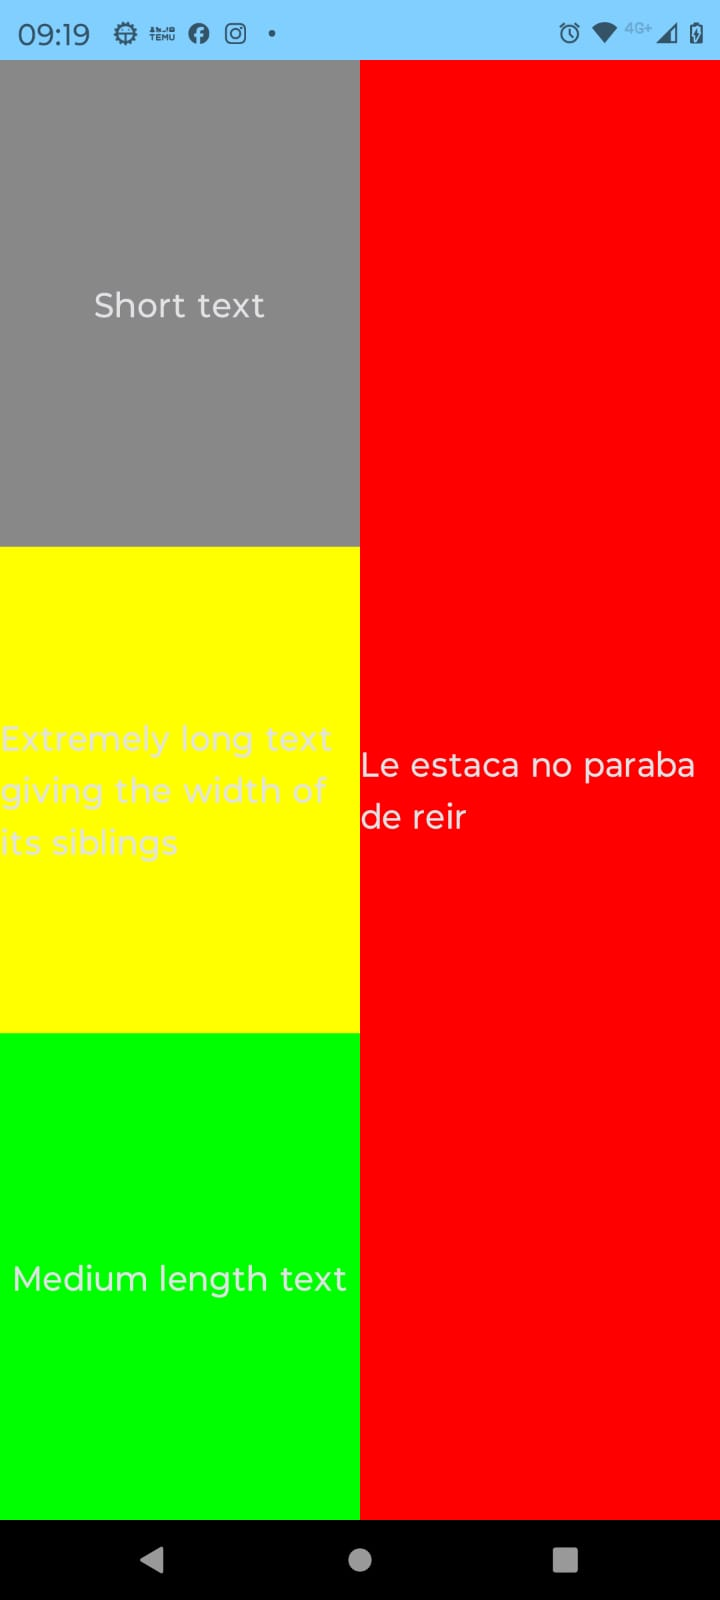
\includegraphics[width=0.98\columnwidth]{graphics/Screenshot3.jpg}       
\end{center}


\end{columns}



    
\end{frame}
\begin{frame}[fragile]

\todo{En codigos muy largos, las lineas deben ir enumeradas}
    \frametitle{Adding Button and EditText (1)}
    \begin{minted}[fontsize=\tiny,linenos]{Kotlin}
@Composable
fun LinearLayout1() {
    val mContext = LocalContext.current
    var clickCount by remember { mutableIntStateOf(0) }
    val mutableList = remember { mutableStateListOf<String>()}
    var text by rememberSaveable { mutableStateOf("") }
    var cadenota  by rememberSaveable { mutableStateOf("") }

    Column(Modifier.width(IntrinsicSize.Max)) {
		Box(Modifier.fillMaxWidth().background(Color.Cyan).
			weight(2.0f).wrapContentSize(Alignment.Center)) {
			Button(
				onClick = {
				    clickCount++
				    mToast(mContext,"Added Element: "+text)
				    mutableList.add(text)
				    cadenota=""
				    var indice: Int = 0
				    while (indice<clickCount) {
				        cadenota += mutableList.toList()[indice] +"\n"
				        indice=indice+1
				    }
				    text=""},
				colors = ButtonDefaults.buttonColors(Color.Gray)
			) {
				Text(text = "SignUp")
			}
		}
\end{minted}
\end{frame}
\begin{frame}[fragile]
    \frametitle{Adding Button and EditText (2)}
    \begin{minted}[fontsize=\tiny,linenos,firstnumber=29]{Kotlin}
		Box(Modifier.fillMaxWidth().background(Color.Yellow).
				weight(2.0f).wrapContentSize(Alignment.Center)) {
				TextField(
					value = text,  onValueChange = { text = it },
					label = { Text("Enter your text") },
					modifier = Modifier.fillMaxWidth() )
			}
			Box(Modifier.fillMaxWidth().background(Color.Red).
				weight(2.0f)) {
				Text(text = "Hello !")
			}
			Box(Modifier.fillMaxWidth().background(Color.Green).
				weight(8.0f)) {
				Text( text = "$cadenota!")
			}
		}
}
	\end{minted}
   
\end{frame}


\end{document}

